\chapter{Technical Implementation}
\label{chap:implementation}
This chapter delves into the practical realisation of the CardioSync framework, translating the architectural concepts and design discussed in the previous chapters into tangible code and functional components. 

\section{Hardware and Software Setup}
This section outlines the necessary hardware setup and software environment required for the implementation of the framework.

\subsection{Hardware Setup}

\noindent Integral part of the devised framework is the heart rate sensor. After a comprehensive review of available low-power heart rate detection sensors in the market, the MAX30102 sensor from Maxim Integrated \cite{2018MAX30102} was selected as the heart rate monitor for the CardioSync framework. The MAX30102 sensor, consuming as less as 1 mW and featuring low shutdown current around 0.7 \(\mu\)A, fits seamlessly with CardioSync's design goals \cite{2018MAX30102}.
\vspace{1\baselineskip}

\noindent The CardioSync framework is built upon the FreeBie model, integrating the MAX30102 sensor. The hardware setup comprises the following components:

\begin{figure}[t]
    \centering
    \includegraphics[width=0.6\linewidth]{chapters/Implementation/FreeBie.png}
    \caption{FreeBie mote (front side). A total size is 1”×1”. A: BLE ARM-based MCU - nRF52840, B: External RTC - AM1815, C: OPT3004 luminosity sensor, D: BMA400 accelerometer, E: BQ25570 energy harvester, F: Two parallel 7.5 mF capacitors, G: , MB85RS4MT fast non-volatile Ferroelectric Random Access Memory (FRAM), H: External power switch, I: SN74AUP2G79 flip-flop that allows the display to stay on when the MCU is off, J: Logic/switches prevent always-on signals from reaching the MCU when its OFF. \cite{de2022Intermittently}.}
    \label{fig:freebie}
\end{figure}

\begin{figure}[t]
    \centering
    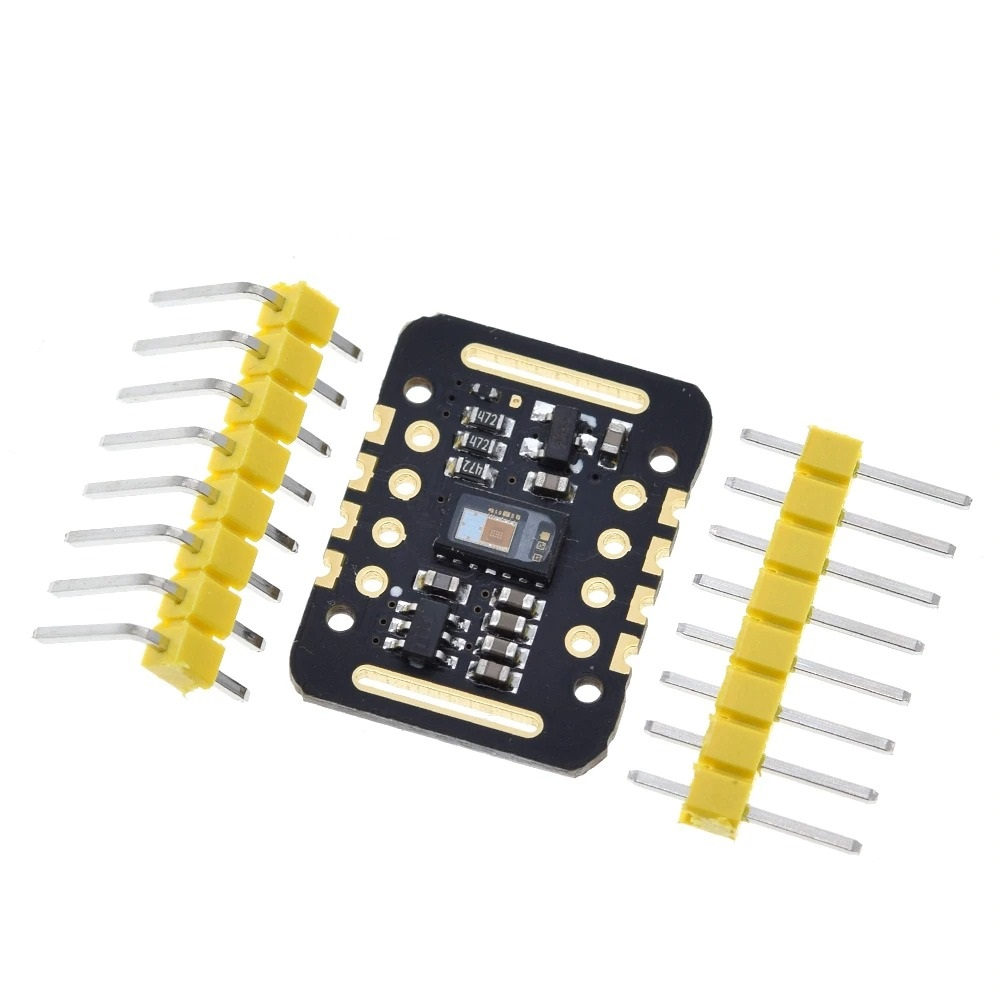
\includegraphics[width=0.4\linewidth]{chapters/Implementation/MAX30102.jpg}
    \caption{MAX30102 sensor module (front side). The pin out marked are VIN: Module power supply 1.8V to 5V; GND: Ground; SCL: I2C clock bus; SDA: I2C data bus \cite{max30102pinout}.}
    \label{fig:max30102}
\end{figure}

\begin{itemize}
    \item \textbf{FreeBie Mote:} This custom board in \autoref{fig:freebie} incorporates essential components, including the nRF52840 ARM-Based MCU module (\textit{EYSKBNZWB}) with BLE radio support, the External RTC and power management module (\textit{AB1815}), and FRAM (\textit{MB85RS4MT}) \cite{de2022Intermittently}. These components provide the foundation for the framework's intermittent operation.
    
    \item \textbf{MAX30102 Sensor Board:} The MAX30102 sensor board from Maxim Integrated, shown in \autoref{fig:max30102}, serves as a critical element for heart rate monitoring. The sensor board features built-in pull-up resistors of 4.7k\(\Omega\) in the \(\text{I}^2\text{C}\) pin outs \cite{2018MAX30102}. However, we noticed even when MCU is in power save or sleep state, instead of near zero voltage and current, a considerable voltage difference of 1.6 Volts in $V_{\text{DD\_MCU}}$ and a current of 1.8mA is drawn by those external pull up resistors. For that reason, sensor's resistors were removed and instead the on-board pull up resistors of the nRF52840 were employed through Software configuration \cite{2021nrf52840pullup}.
    
    \item \textbf{Connection Configuration:} Based on the pinout configuration of the FreeBie schematics \cite{FreeBieGithub},  \(\text{I}^2\text{C}\) Clock Line (SCL) and \(\text{I}^2\text{C}\) Data Line (SDA) of the MAX30102 is connected to the respective GPIO pins. The MAX30102 is powered by the onboard super capacitors, connected to the $V_{\text{Batt}}$ pinout of the FreeBie Mote.
\end{itemize}

\subsection{Software Setup}
\label{sec:software_setup_impl}
The implementation of the CardioSync framework builds upon the open-source FreeBie source code, available from the TU Delft Sustainable Systems Lab repository \cite{FreeBieGithub}. The adaptation process involves customising the existing \textit{"template"} application to accommodate the CardioSync system architecture  - MAX30102 sensor and the Heart Rate peak detection algorithm.

\subsubsection{Software Foundation and Customisation}

The entire FreeBie source code relies on the PacketCraft BLE stack \cite{2020Packetcraft}, which seamlessly integrates nRF5 SDK libraries for driver interfaces and peripheral interactions \cite{2023nRF5}. The code is specifically tailored for the nRF52840 MCU, utilising the GNU ARM Embedded toolChain, thus eliminating the need for additional build support or toolchain.

\subsubsection{Sensor Interfacing}

For interfacing with the MAX30102 sensor, nRFx driver for the Two Wire Interface - Master (TWIM) is employed. This involves enabling the necessary configurations in the \textit{sdk\_config.h} file of nRF5 SDK to activate the TWIM in the system. Subsequently, relevant APIs provided by the nRFx library are utilised for reading from and writing to the \(\text{I}^2\text{C}\) interface.
 
\subsubsection{BLE Stack Configuration}

In the context of the BLE stack, PacketCraft's CMake configurations take charge of initialising the MCU as either a Peripheral or Central device. Two specific CMake definitions, namely \texttt{INIT\_PERIPHERAL} and \texttt{INIT\_CENTRAL}, determine the operational mode. PacketCraft then leverages essential components like the \textit{Device Manager} and the \textit{Application framework main module} to initialise the BLE stack. This equips the framework with APIs that helps with the initiation and termination of advertising or scanning activities depending on whether the device is operating as a Peripheral or Central.

\subsubsection{Timing and Scheduling}
\label{sec:wsf_apptimer}
Both the FreeBie and CardioSync frameworks require precise timing and scheduling mechanisms. PacketCraft's Wireless Software Foundation (WSF) OS layer offers essential APIs for managing the AppTimer functionality. AppTimer is essentially a timer management module that allows to schedule and manage various timing events and callbacks within the application. It provides a way to create, start, stop, and manage timers, which can be crucial to perform real-time tasks at specific intervals.
\vspace{1\baselineskip}

\noindent In the context of your CardioSync framework, WSF AppTimer was utilised to handle timing-related operations such as to schedule the sampling of the heart rate sensor at the desired frequency. It also ensures that BLE connection setup occur at the right times and in synchronisation with each other. 
\vspace{1\baselineskip}

\noindent Additionally, these WSF AppTimer aid in the FreeBie architecture's ability to accurately track the timing of active scheduled tasks inside the queue. Consequently, the system is able to power down and enter a sleep state when there are no planned activities for the next period. 


\section{Sensor Interface and Peak Detection Algorithm}
\label{sec:sensor_data_impl}
This section delves into the practical implementation and methodologies used for interfacing the MAX30102 sensor with the FreeBie architecture and the novel heart rate peak detection algorithm.
\vspace{1\baselineskip}

\noindent As outlined in the section \ref{sec:software_setup_impl}, the existing "template" application within the FreeBie source code is extended to incorporate the MAX30102 sensor functionality into a new source file which houses all the necessary functions, declarations, and configurations.

\subsection{MAX30102 Sensor Data Acquisition}

\begin{algorithm}[t]
\caption{MAX30102 Sensor Data Acquisition}
\scriptsize
\label{alg:sensor_data_collection}
\begin{algorithmic}[1]

\State Initialize 2D Buffer with maximum capacity of 2 x 500
\State Initialize Sliding Window size as 10
\item[]
\State Start "\textit{\texttt{MAX30102Timer}}" with 10 milliseconds period \Comment{After converting sampling rate: 100 Hz into milliseconds (\(1000 / Sampling Rate\))}
\item[] 
\If{\textit{\texttt{MAX30102Timer}} expired}
    \State Read MAX30102 sensor's FIFO using "\texttt{MAX30102\_read\_fifo()}" \Comment{Called from Timer Expiry event handling}
    \State Append IR value and corresponding RTC ticks to 2D Buffer and Sliding Window
    \item[] 
    \If{Sliding Window is full and Average of sample data > 8000}
        \State Call Heart Rate Peak Detection API on Sliding Window data \Comment{\texttt{calculate\_heart\_rate()}}
    \EndIf
    \item[] 
    \State Restart "\textit{\texttt{MAX30102Timer}}"
\EndIf

\end{algorithmic}
\end{algorithm}

Before starting the sensor sampling, sensor should be initialised and configured with settings that ensures optimal performance while minimising power consumption. Different configuration settings done for MAX30102 is described in detail in Section \ref{sec:sensor_config} of Appendix \ref{app:appendix_a}. With these settings, MAX30102 operates with less power consumption, yet capturing accurate blood flow for heart rate analysis.
\vspace{1\baselineskip}

\noindent This section outlines the methodology employed for data collection, using buffers and sliding window within the CardioSync framework. The process of the data acquisition is given in Algorithm \ref{alg:sensor_data_collection}.
\vspace{1\baselineskip}

\noindent The raw data is continuously read from the MAX30102 sensor's FIFO at a predetermined sampling rate of 100 Hz. This sampling rate of 100 Hz is chosen after thorough evaluation of sensor which will be covered in Section \ref{sec:sensor_performance}. 
\vspace{1\baselineskip}

\noindent A two dimensional buffer named "\texttt{ir\_values}" with a maximum capacity of 2 x 500 entries is employed to store the sensor data and their respective RTC ticks at which they are read. Also a sliding window named "\texttt{window}" of size 10 is chosen, to store the latest 10 sensor values at any instance.
\vspace{2\baselineskip}

\noindent Now that the initial setup and configurations are laid out, the data acquisition process is orchestrated by the following key steps:

\begin{enumerate}
    \item \textbf{Start of the Sampling:} A WSF Apptimer named \texttt{MAX30102Timer} is started to start the sampling of MAX30102 sensor. The timer's period is determined to be 10 milliseconds i.e., \(1000\) divided by the chosen sampling rate of 100Hz. 

    \item \textbf{FIFO Read and Buffering:} When the timer expires, the sensor's FIFO is read using the "\texttt{MAX30102\_read\_fifo()}" function. This function relies on the \texttt{nrfx\_twim} driver APIs to extract the real-time IR value that holds blood flow data for heart rate peak detection. Consequently, it is paired with the corresponding RTC ticks at the time which it was recorded and appended to the end of the 2-D buffer, i.e., \texttt{ir\_values} buffer and also to the \texttt{window} buffer.

    \item \textbf{Continuous Data Acquisition:} The "\texttt{MAX30102Timer}" is restarted and the sequence repeats till the timer is stopped or not started again. This ensures the raw data from sensor is continuously read and latest 10 values always stay in the \texttt{window} buffer. When the \texttt{ir\_values} buffer becomes full, it undergoes a rotation where the samples are shifted to the left, causing the oldest value to be discarded. Subsequently, the newest value is appended to the right end of the buffer. 
    
    \item \textbf{Ready for peak detection:} This happens when the sliding window buffer - \texttt{window} is full. The data is subjected to heart rate peak detection algorithm only if the average of the data within the sliding window surpasses the threshold of 8000. This threshold was determined after analysing the sensor's raw data, which showed consistent changes when the sensor was in proximity to human skin compared to when it was not. After configuring the sensor, it recorded values above 8000 when in contact with human skin. Thus, this threshold ensures peak detection happens when the sensor reliably maintains contact with the skin.
\end{enumerate}

\noindent The iterative nature of this process guarantees the availability of up-to-date sensor data for real-time heart rate analysis, ensuring the responsiveness and accuracy of the CardioSync system.


\subsection{Heart Rate Peak Detection Algorithm}
\label{sec:heart_rate_algo_impl}

\begin{figure}[t]
    \centering
    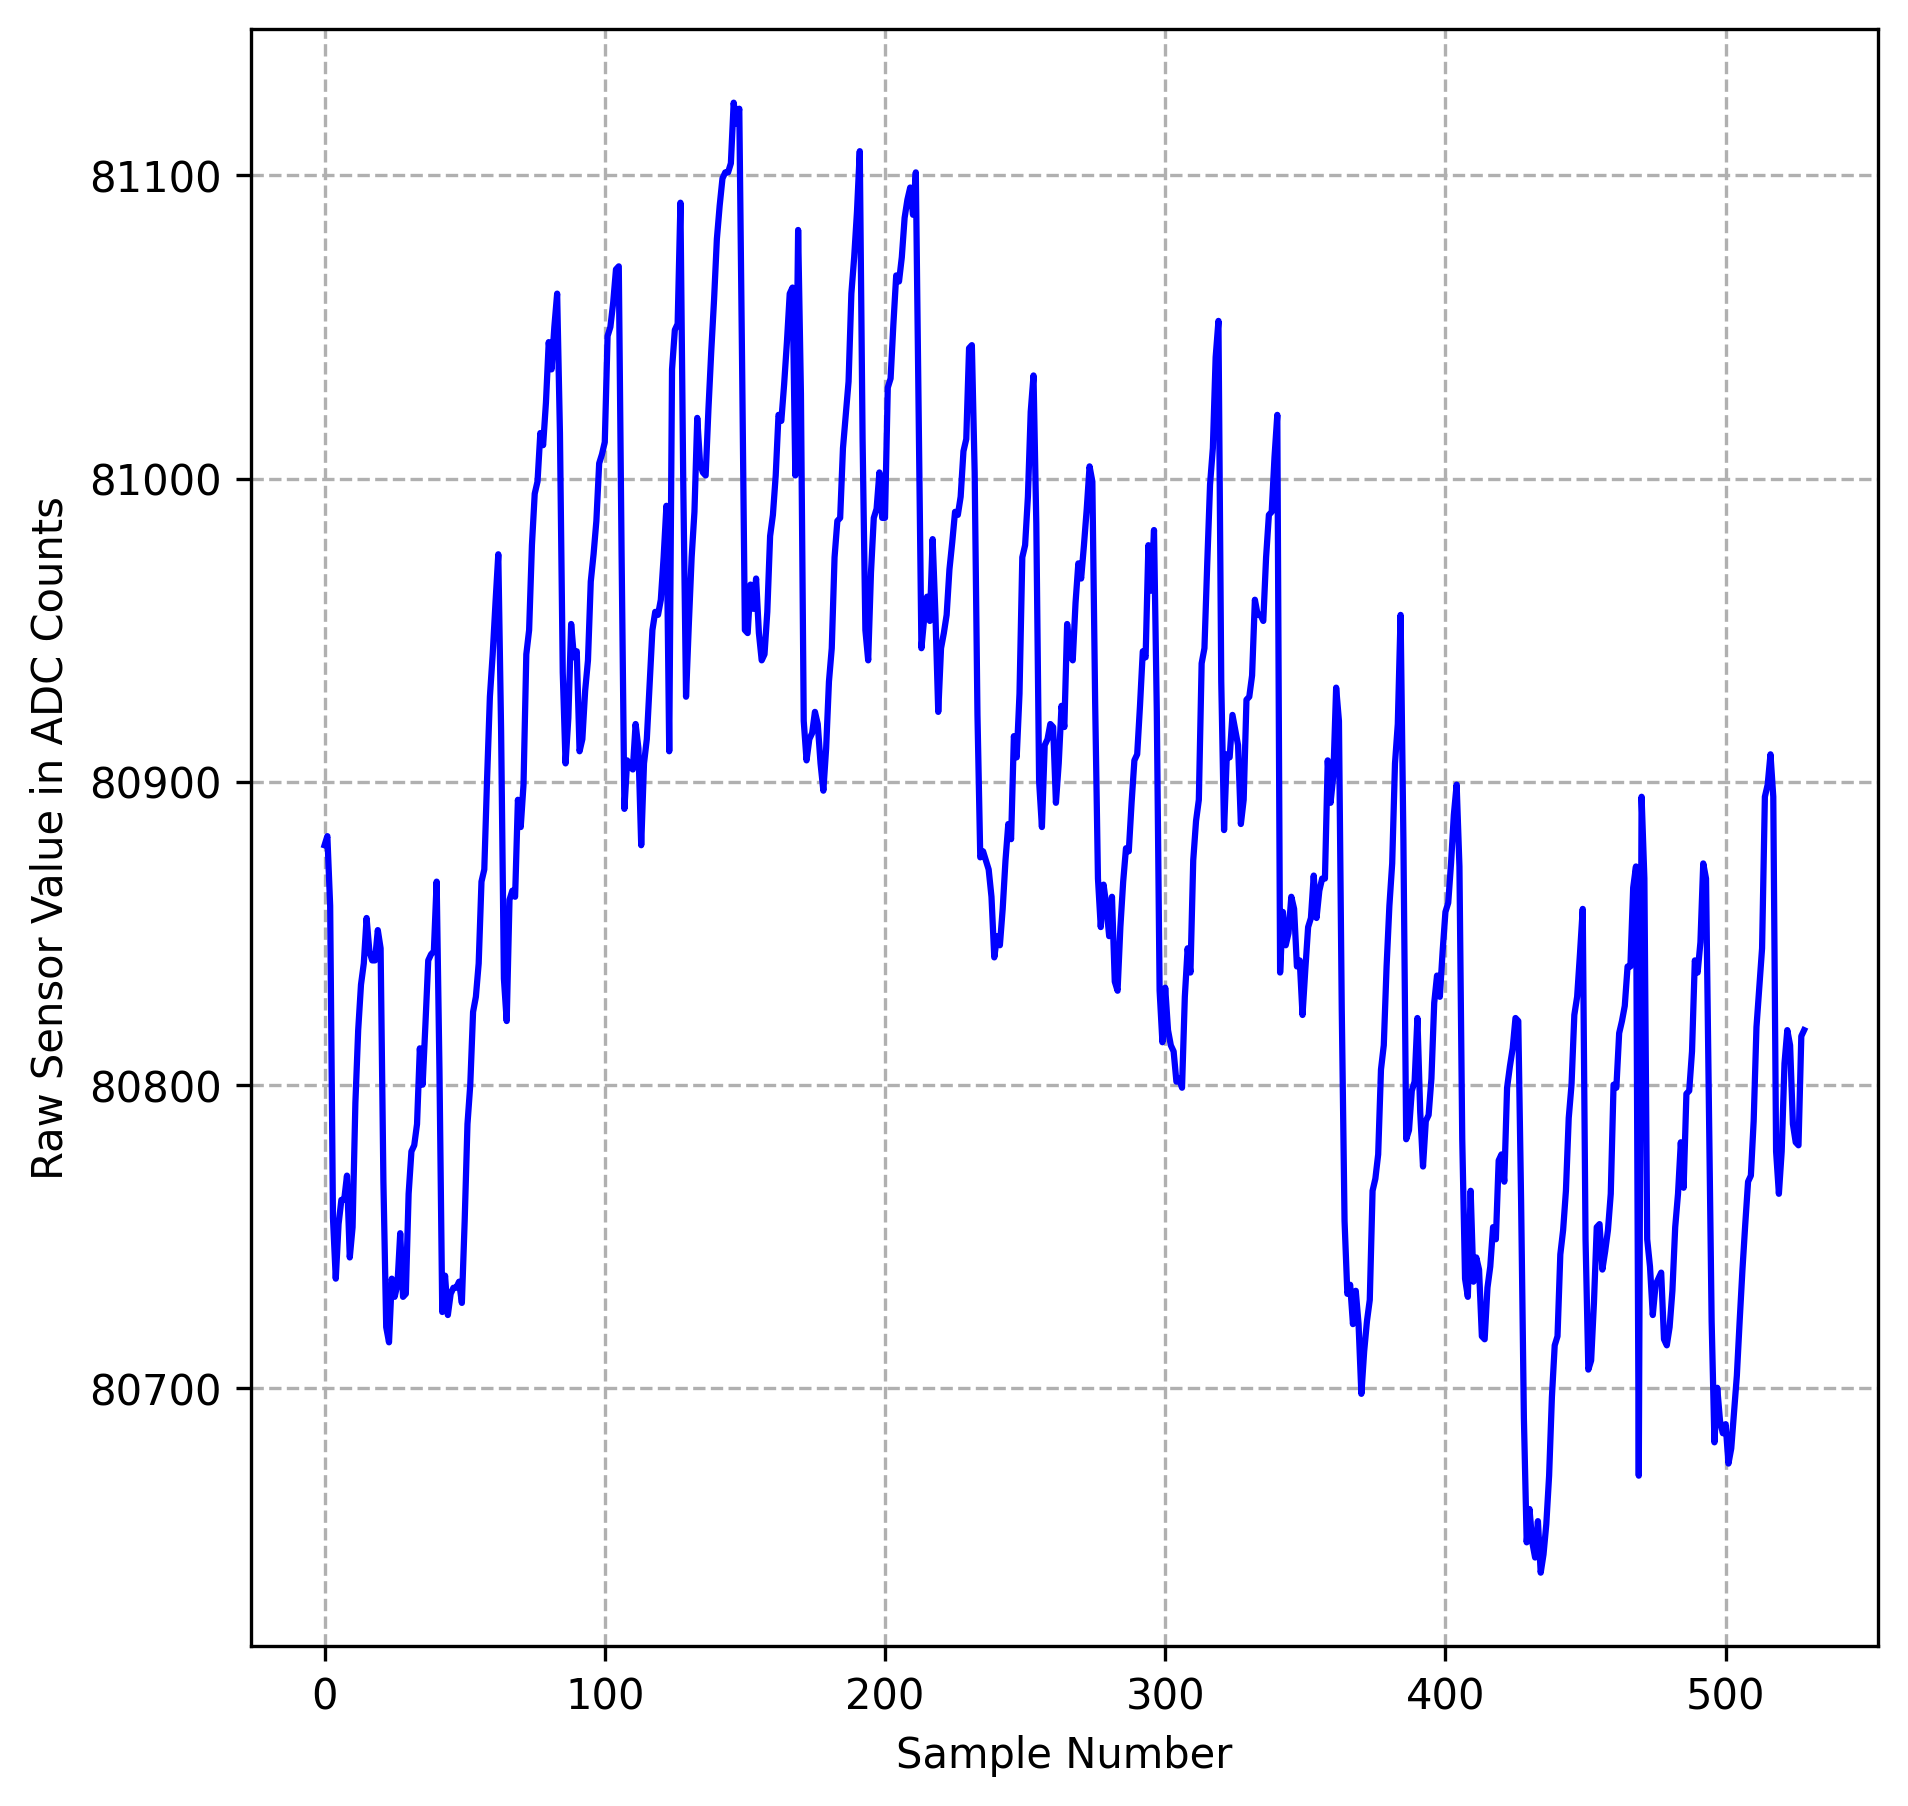
\includegraphics[width=0.7\linewidth]{chapters/Implementation/dynamic_threshold.png}
    \caption{Example measurement showing the dynamic and fluctuating nature of continuous sensor data readings from MAX30102. The Y-axis represents the sensor's raw data in ADC count units. These units indicate the magnitude of the analog signal measured by the sensor and converted into digital form by the analog-to-digital converter (ADC).}
    \label{fig:dynamic_threshold}
\end{figure}
\noindent Initially, an attempt was made to utilise Maxim Integrated's reference heart rate peak detection algorithm \cite{SparkFun_MAX3010x_Sensor_Library} developed for their low power, optical heart-rate module - MAXREFDES117 \cite{2016maxrefdes117}. This algorithm employed a method of peak identification by calculating a fixed threshold and detecting peaks above that threshold. However, this approach proved ineffective for the CardioSync framework due to the dynamic and varying nature of the continuous sensor data readings obtained from the MAX30102. As shown in Figure~\ref{fig:dynamic_threshold}, the sensor data exhibited fluctuations that necessitated a more adaptive and dynamic threshold approach.
\vspace{1\baselineskip}

\noindent In light of these challenges, the decision was made to adopt an alternative approach that leverages the derivatives of the sensor data for peak detection. This approach was more suitable for handling the varying nature of the sensor readings and provided a robust means of detecting heart rate peaks.
\vspace{1\baselineskip}

\noindent The heart rate peak detection algorithm using derivatives operates as follows:

\begin{enumerate}
    \item \textbf{Data Preprocessing:} The raw sensor data collected from Sliding window buffer, denoted as \texttt{\(\text{a}_\text{ir}\)}, undergoes preprocessing steps. The algorithm removes the DC component by calculating the mean and subtracting it from the data. This step is essential to eliminate any static offset and focus on the variations caused by heartbeats.
    
    \item \textbf{Moving Average:} The \texttt{\(\text{a}_\text{ir}\)} data is then updated using a moving average of two neighbouring samples on either side of each sample. This smoothing technique helps reduce noise and sharp variations in the data, facilitating more accurate peak detection.
    
    \item \textbf{Derivative Calculation:} The first derivative of the \texttt{\(\text{a}_\text{ir}\)} data, referred to as \texttt{\(\text{a}_\text{ir\_diff}\)}, is calculated. This derivative provides insights into the rate of change of the signal, which is particularly useful for identifying rapid transitions characteristic of heart rate peaks.
    
    \item \textbf{Peak and Valley Detection:} The algorithm identifies peaks and valleys within the \texttt{\(\text{a}_\text{ir\_diff}\)} data. Peaks correspond to points where the derivative changes from positive to negative, indicating a downward slope. Valleys, conversely, represent points where the derivative changes from negative to positive, indicating an upward slope. These points mark significant variations in the signal, which are indicative of heart rate peaks.
    
    \item \textbf{Peak Validation and Removal:} Detected peaks that are in close proximity to valley indices are discarded. A maximum distance threshold \textbf{\texttt{n\_valley\_distance}} of value \textbf{4} is used to determine this proximity. Similarly, peaks that are too close to each other, within a distance threshold \textbf{\texttt{n\_peak\_distance}} of value \textbf{15}, are also removed. The selection of these thresholds is based on the retrospective analysis of visual patterns on the continuous sensor read. The visual analysis helped to determine the typical distances between peaks and the lengths between valleys and subsequent peaks. These additional validation steps help ensure that the detected peaks correspond to distinct heart rate events.
    
    \item \textbf{Result Generation:} The algorithm generates a list of validated peak indices that represent heart rate peaks which likely to have occurred.
    
    \item \textbf{Callback and Post Processing:} For each detected and validated peak index, the algorithm invokes the \texttt{sensor\_callback} function. This function handles further processing, synchronisation, and scheduling tasks related to the CardioSync framework.
\end{enumerate}

\noindent The constants \texttt{n\_valley\_distance}, and \texttt{n\_peak\_distance} are empirically determined based on the characteristics of the sensor data and the expected heart rate patterns. These values ensure the reliability and accuracy of the peak detection process. The algorithm is outlined in Algorithm \ref{alg:heart_rate_algorithm}

\begin{algorithm}[ht]
\footnotesize
\caption{Heart Rate Peak Detection Algorithm}
\label{alg:heart_rate_algorithm}
\begin{algorithmic}[1]
\Function{calculate\_heart\_rate}{$a\_ir, callback$}
    \item[] \Comment{{\scriptsize $a\_ir$: array of sensor data from Sliding window buffer.}}
    \item[] \Comment{{\scriptsize $callback$: callback function to process the peaks detected by algorithm.}}
\item[]
    
    \State Initialise  $a\_ir\_clean[ ]$, $a\_ir\_diff[ ]$, $peak\_indices[ ]$, and $valley\_indices[ ]$
    \item[] \Comment{{\scriptsize $a\_ir\_clean[ ]$: array of sensor data after DC component is removed}}
    \item[] \Comment{{\scriptsize $a\_ir\_diff[ ]$: array of first derivative of sensor data}}
    \item[] \Comment{{\scriptsize $peak\_indices[ ]$: array of detected peak indices in the sensor data}}
    \item[] \Comment{{\scriptsize $valley\_indices[ ]$: array of detected valley indices in the sensor data}}
\item[]

    \State $\mu = \frac{1}{n}\sum_{i=1}^{n} a\_ir[i]$ \Comment{{\scriptsize Calculate mean of raw IR sensor data}}
    \item[] \Comment{{\scriptsize n: size of $a\_ir$ array, which is 10 (size of sliding window buffer)}}
\item[]

    \For{each data point $x$ in $a\_ir$} \Comment{{\scriptsize Removing DC component in sensor data}}
        \State $a\_ir\_clean[x] = a\_ir[x] - \mu$
    \EndFor
\item[]

    \For{each data point $x$ in $a\_ir\_clean$} \Comment{{\scriptsize Filtering out sensor data using moving average of two neighbouring data on both side of each data point}}
        \State $a\_ir\_clean[x] = \frac{1}{5}\sum_{i=x-2}^{x+2} a\_ir\_clean[i]$
    \EndFor
\item[]

    \For{each data point $x$ in $a\_ir\_clean$}
 \Comment{{\scriptsize First derivative of sensor data}}
        \State $a\_ir\_diff[x] = a\_ir\_clean[x] - a\_ir\_clean[x-1]$
    \EndFor
\item[]

    \For{each index $x$ in range $1$ to $n - 2$}
\Comment{{\scriptsize Peak detection}}
        \If{$a\_ir\_diff[x - 1] > 0$ \textbf{and} $a\_ir\_diff[x] < 0$}
            \State $peak\_indices[ ] \gets x$
        \EndIf
    \EndFor
\item[]

    \For{each index $x$ in range $1$ to $n - 2$}
\Comment{{\scriptsize Valley detection}}
        \If{$a\_ir\_diff[x - 1] < 0$ \textbf{and} $a\_ir\_diff[x] > 0$}
            \State $valley\_indices[ ] \ge x$
        \EndIf
    \EndFor
\item[]

    \State Remove peaks close to each other using $n\_peak\_distance$ threshold
    \State Remove peaks close to valleys using $n\_valley\_distance$ threshold
\item[]

    \State Call $callback$ function with detected peak indices to process them
    
\EndFunction
\end{algorithmic}
\end{algorithm}

\section{CardioSync Integration with FreeBie BLE}
\begin{figure}[t]
    \centering
    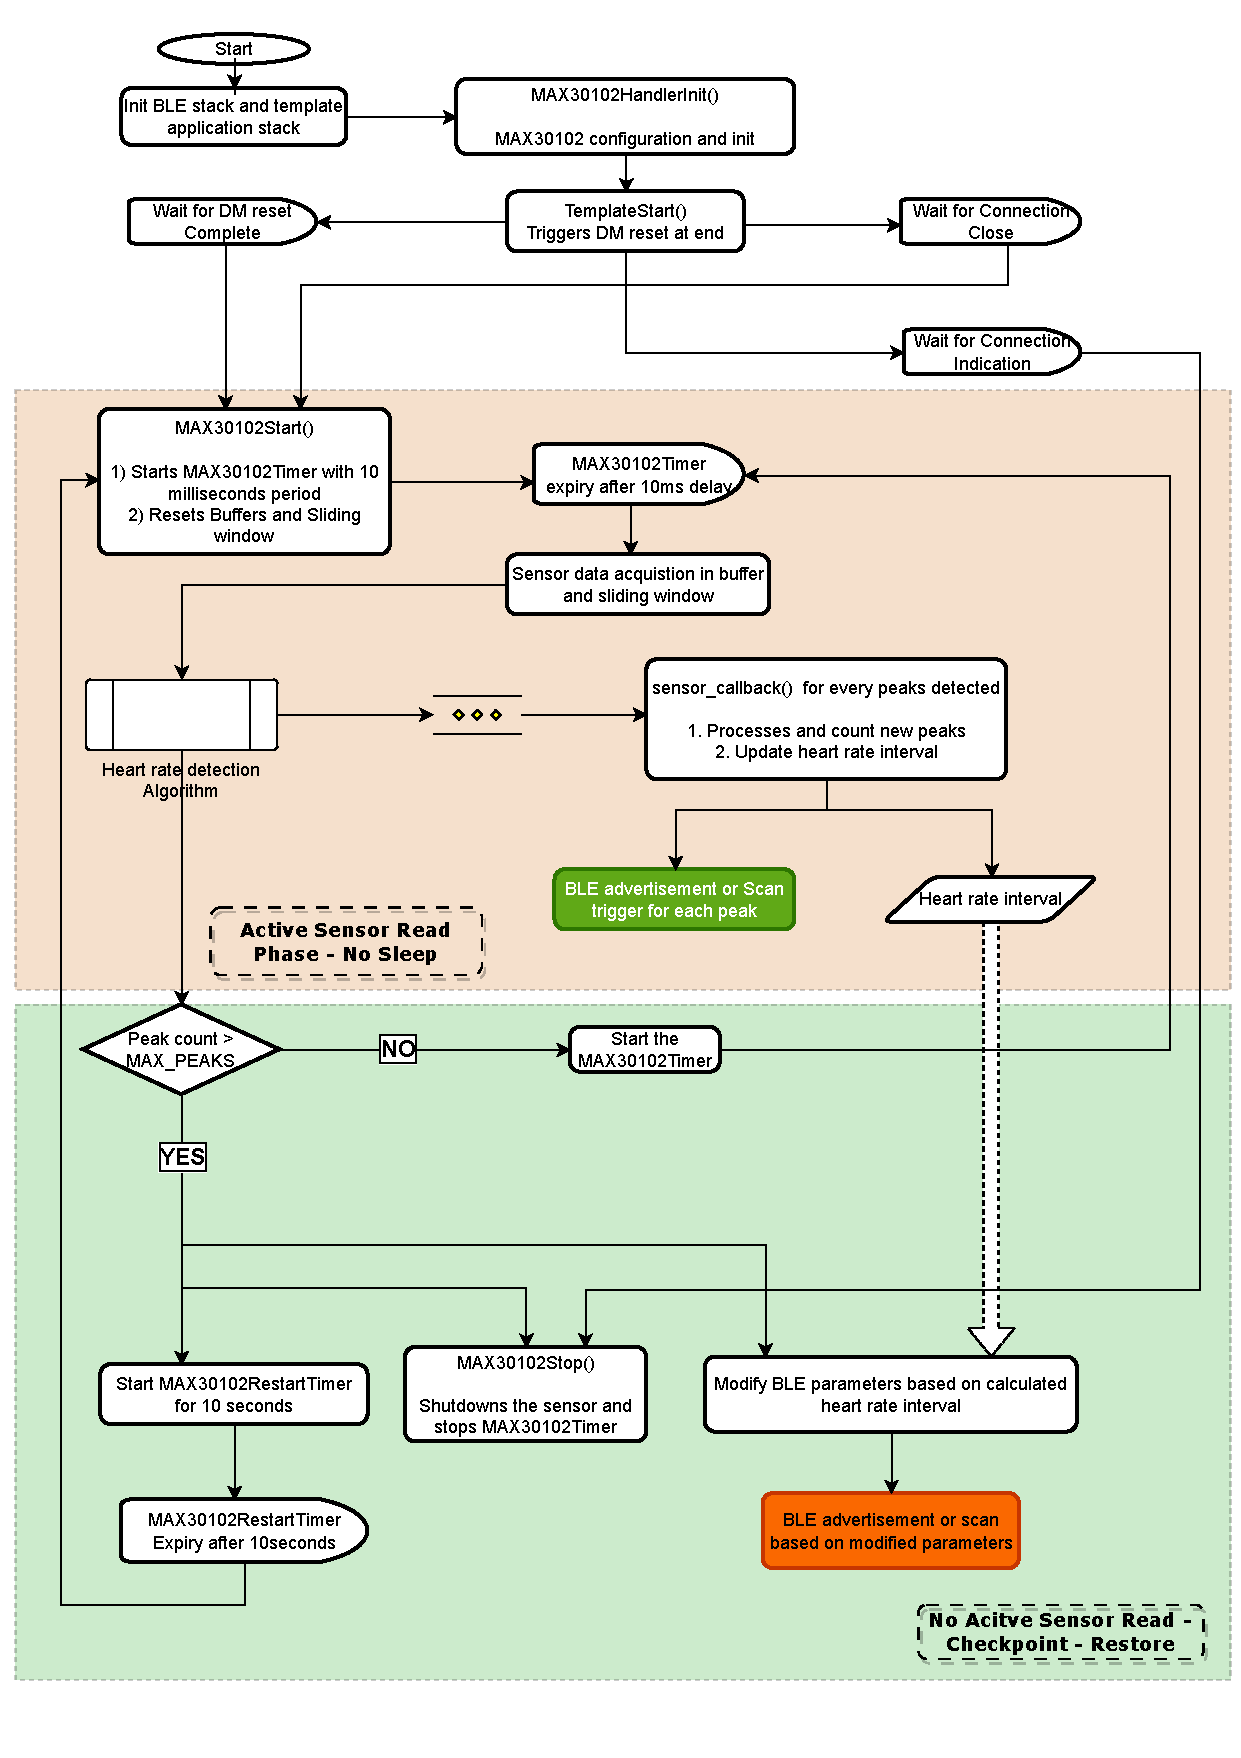
\includegraphics[width=\linewidth]{chapters/Implementation/Flowchart_CardioSync.pdf}
    \caption{Operation flowchart of the CardioSync framework implementation.}
    \label{fig:flowchart}
\end{figure}


With the fundamental components of the CardioSync framework described, the next step involves integrating these elements into the FreeBie architecture. This section provides insight into how these various parts work together to create a functional system, ensuring accurate heart rate peak detection and synchronised BLE connection setup within a battery less system architecture.
\vspace{1\baselineskip}

\noindent An effective approach to elucidate the integration within FreeBie is to follow the chronological flow of steps required for establishing a synchronised BLE connection from a coding perspective. This approach is represented as a flowchart in Figure \ref{fig:flowchart}.


\subsubsection{System Initialisation}
Starting from the beginning of the execution process, depending on whether the device operates in a peripheral or central mode, the necessary BLE modules of the FreeBie architecture are initialised within the "template" application's stack initialisation. The initialisation of the CardioSync extension framework, which includes the MAX30102 sensor, is also integrated into the stack initialisation process.
\vspace{1\baselineskip}

\noindent The MAX30102 initialisation manages the setup and configuration of the sensor, as described in Section \ref{sec:sensor_config} of Appendix \ref{app:appendix_a}. Additionally, the essential WSF AppTimers as explained in Section \ref{sec:wsf_apptimer}, such as \texttt{MAX30102Timer} and \texttt{MAX30102RestartTimer}, are declared and initialised in this process. The specific roles and functions of these timers will be further explained. 

\subsubsection{Sensor Data Acquisition and Peak Detection}
With all essential initialisation have been accomplished, the sampling of sensor is started through \texttt{MAX30102Start()} function, which kicks off the \texttt{MAX30102Timer} timer and starts the process of data acquisition and heart rate peak detection which was \ref{sec:sensor_data_impl} and \ref{sec:heart_rate_algo_impl}.

\subsubsection{Read and Synchronise}
With the successful identification of heart rate peaks, the post processing is rudimentary to distinguish between new peaks and peaks that linger within the rotating 2-D buffer. This differentiation is achieved by utilising the RTC ticks associated with the detected peak indices.
\vspace{1\baselineskip}

\noindent Additionally, as new peaks are identified, the post-processing routine updates the average time difference between peaks in a global variable - the \textit{"Heart Rate Interval"}. This value later holds significant importance in establishing synchronisation points based on heart rate.
\vspace{1\baselineskip}

\noindent Depending on the operational mode of the system, either advertisement or scan initiation is executed as soon as a new peak is detected using PacketCraft's APIs, such as \texttt{AppAdvStart()} or \texttt{AppScanStart()}.  These APIs use the BLE parameters that are strategically chosen based on the comprehensive evaluation of algorithm performance and system behaviour outlined in Table \ref{tab:ble_params}. It is noteworthy that this synchronised BLE connection setup operates simultaneously with continuous sensor read at a 100Hz sampling rate and heart rate peak detection.

\subsubsection{Sleep and Synchronise}

% \begin{table}[t]
% \centering
% \begin{tabular}{|cc|}
% \hline
% \multicolumn{2}{|c|}{\textbf{\begin{tabular}[c]{@{}c@{}}BLE Advertisement Parameters\\ (Peripheral)\end{tabular}}} \\ \hline
% \multicolumn{1}{|c|}{\textit{Advertising Interval}} & Heart rate interval \\ \hline
% \multicolumn{1}{|c|}{\textit{Advertising Duration}} & 10 seconds          \\ \hline
% \multicolumn{2}{|c|}{\textbf{\begin{tabular}[c]{@{}c@{}}BLE Scan Parameters\\ (Central)\end{tabular}}}             \\ \hline
% \multicolumn{1}{|c|}{\textit{Scan Interval}}        & Heart rate interval \\ \hline
% \multicolumn{1}{|c|}{\textit{Scan Window}}          & 100 milliseconds    \\ \hline
% \multicolumn{1}{|c|}{\textit{Scan Duration}}        & 10 seconds          \\ \hline
% \end{tabular}
% \caption{Modified BLE parameters during runtime based on calculated heart rate interval (\texttt{average\_time\_diff})}
% \label{tab:modified_ble_params}
% \end{table}


\noindent After the detection of three peaks (\texttt{MAX\_PEAKS}), the \texttt{MAX30102Stop()} routine is invoked. It shuts down the sensor by configuring the power-saving mode and terminates \texttt{MAX30102Timer}, thereby suspending active sensor read and heart rate peak detection. BLE parameters are also then dynamically adjusted during runtime to ensure the scheduling of advertisement or scanning events aligned with the global variable \textit{Heart Rate Interval}. The modified BLE parameters are:
\begin{itemize}
    \item \textbf{BLE Advertisement Parameters (Peripheral):}
        \begin{itemize}
            \item Advertising Interval is adjusted runtime with global variable \textit{Heart Rate Interval}.
            \item Advertising Duration is 10 seconds.
        \end{itemize}
    \item \textbf{BLE Scan Parameters (Central):}
        \begin{itemize}
            \item Scan Interval is modified in runtime with global variable \textit{Heart Rate Interval}.
            \item Scan Window is fixed as 100 milliseconds.
            \item Scan duration is set as 10 seconds.
        \end{itemize}
\end{itemize}

\noindent The incorporation of \textit{Heart Rate Interval} in BLE parameters establishes the fixed synchronisation points for the system without any active sensor read. The scheduling of BLE connection events only during the established synchronisation points, results in the system being idle without any active tasks during the \textit{Heart Rate Interval} period. The Checkpointing and Restore module, which is integrated into the FreeBie architecture, identifies system inactivity and utilises checkpointing to preserve the current state of the system while temporarily halting the operations of the MCU. The system resumes its operation at predetermined BLE synchronisation points and recovers its context, after which it returns to a sleep state for the upcoming heart rate period.


\subsubsection{Adaptive Heart Rate Update}
In cases where the BLE connection setup experiences prolonged delays, the continuity of the \textit{Heart Rate Interval} may become compromised. In response, an adaptive iterative strategy is employed. A timer, \texttt{MAX30102RestartTimer}, restricts the "Sleep and Synchronise" phase to a 10-second duration. Upon the timer's expiration, \texttt{MAX30102Start()} is called again, triggering the "Read and Synchronise phase" which updates \textit{Heart Rate Interval}. The iterative process between phases is stopped once a successful BLE connection is established. Additionally, when the connection is closed, \texttt{MAX30102Start()} is reinvoked to start "Read and Synchronise" phase. 
